\documentclass{standalone}
\usepackage[dvipsnames]{xcolor}
\usepackage{tikz}
\usepackage{fix-cm}
\usepackage{libertine}
\setlength{\parskip}{0pt}
\setlength{\baselineskip}{0pt}
%\usetikzlibrary{fit}
\usetikzlibrary{calc}
\usetikzlibrary{decorations.markings}
\usetikzlibrary{decorations.shapes}
\usetikzlibrary{decorations.pathreplacing}
\usetikzlibrary{intersections}
\usetikzlibrary{patterns}
\newcommand{\liy}{-0.3}
\newcommand{\giy}{-0.6}
\tikzset{%
  from end of path/.style={
    insert path={
      \pgfextra{%
        \expandafter\pgfprocesspathextractpoints%
          \csname tikz@intersect@path@name@#1\endcsname%
        \pgfpointlastonpath%
        \pgfgetlastxy\lastx\lasty
      }
      (\lastx,\lasty)
}}}
\tikzset{-dot-/.style={decoration={
  markings,
  mark=at position #1 with {\fill[color=red] circle (0.5mm);}},postaction={decorate}}}  
\tikzset{-dot2-/.style={decoration={
  markings,
  mark=at position #1 with {\draw[color=black] (0,-0.25mm) -- (0,0.25mm); (0.25mm);}},postaction={decorate}}}
    \tikzset{
        hatch distance/.store in=\hatchdistance,
        hatch distance=10pt,
        hatch thickness/.store in=\hatchthickness,
        hatch thickness=2pt
    }
\begin{document}
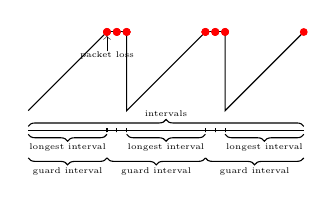
\begin{tikzpicture}
    
    \makeatletter
    \pgfdeclarepatternformonly[\hatchdistance,\hatchthickness]{flexible hatch}
    {\pgfqpoint{0pt}{0pt}}
    {\pgfqpoint{\hatchdistance}{\hatchdistance}}
    {\pgfpoint{\hatchdistance-1pt}{\hatchdistance-1pt}}%
    {
        \pgfsetcolor{\tikz@pattern@color}
        \pgfsetlinewidth{\hatchthickness}
        \pgfpathmoveto{\pgfqpoint{0pt}{0pt}}
        \pgfpathlineto{\pgfqpoint{\hatchdistance}{\hatchdistance}}
        \pgfusepath{stroke}
    }
    \makeatother
 
\draw[name path=A] (0,0)-- ++(1, 1);
\draw[from end of path=A, name path=B, -dot-=0, -dot-=0.5, -dot-=1] -- ++(0.25,0);
\node[align=center,font=\fontsize{3pt}{0}\selectfont,inner sep=0mm] at (1, 0.7) (lossLabel) {packet loss};
\draw[->, line width=0.05mm] (lossLabel) -- (1,0.95);
\draw[from end of path=B, name path=C] ++(0,-0.5mm) -- ++(0,-0.95cm) -- ++(1,1);
\draw[from end of path=C, name path=D, -dot-=0, -dot-=0.5, -dot-=1] -- ++(0.25,0);
\draw[from end of path=D, name path=E, -dot-=1] ++(0,-0.5mm) -- ++(0,-0.95cm) -- ++(1,1);

%\node[anchor=north west,align=left,font=\fontsize{3pt}{0}\selectfont,inner sep=0mm] at (0.5mm, -1mm) (intervalsLabel) {intervals};
\draw[name path=F] (0,-0.25)-- ++(1, 0);
\draw[from end of path=F, name path=G, -dot2-=0, -dot2-=0.5, -dot2-=1] -- ++(0.25,0);
\draw[from end of path=G, name path=H] -- ++(1,0);
\draw[from end of path=H, name path=I, -dot2-=0, -dot2-=0.5, -dot2-=1] -- ++(0.25,0);
\draw[from end of path=I, name path=J] -- ++(1,0);

\draw[draw,decorate,decoration={brace}] (0,-0.2) -- ++(3.5,0) node [,midway,above,font=\fontsize{3pt}{0}\selectfont] {intervals};

\draw[draw,decorate,decoration={brace,mirror}] (0,\liy) -- ++(1,0) node [inner sep=0, outer sep=0,midway,below,yshift=-1.25mm,font=\fontsize{3pt}{0}\selectfont] {longest interval};
\draw[draw,decorate,decoration={brace,mirror}] (1.25,\liy) -- ++(1,0) node [inner sep=0, outer sep=0,midway,below,yshift=-1.25mm,font=\fontsize{3pt}{0}\selectfont] {longest interval};
\draw[draw,decorate,decoration={brace,mirror}] (2.5,\liy) -- ++(1,0) node [inner sep=0, outer sep=0,midway,below,yshift=-1.25mm,font=\fontsize{3pt}{0}\selectfont] {longest interval};

\draw[draw,decorate,decoration={brace,mirror}] (0,\giy) -- ++(1,0) node [inner sep=0, outer sep=0,midway,below,yshift=-1.25mm,font=\fontsize{3pt}{0}\selectfont] {guard interval};
\draw[draw,decorate,decoration={brace,mirror}] (1,\giy) -- ++(1.25,0) node [inner sep=0, outer sep=0,midway,below,yshift=-1.25mm,font=\fontsize{3pt}{0}\selectfont] {guard interval};
\draw[draw,decorate,decoration={brace,mirror}] (2.25,\giy) -- ++(1.25,0) node [inner sep=0, outer sep=0,midway,below,yshift=-1.25mm,font=\fontsize{3pt}{0}\selectfont] {guard interval};

\end{tikzpicture}
\end{document}